\documentclass[a4paper,12pt]{extarticle}
\usepackage[utf8]{inputenc}
\usepackage{graphicx}
\usepackage{natbib}
\usepackage{amsmath}
\usepackage{caption}
\usepackage{subcaption}
\usepackage{geometry}
    \geometry{a4paper}
\bibliographystyle{apalike}


\title{Discovering Focused Microgenre Communities}

\begin{document}
\maketitle
\subsubsection*{Abstract} 
Recent work in the sociology of taste has begun to grapple directly with the relational properties of traditional survey-based data using techniques inspired by network analysis. Despite the generally salutary results from this endeavor, critics rightly question the face and ecological validity of the vague macrogenre labels included in standard arts participation surveys (e.g., Classical, Rock, Rap). To deal with this issue, in this paper, I propose a link-clustering approach for discovering focused microgenres from standard survey-based information on cultural tastes, one that exploits the underlying relational patterns realized by the indirect connectivity structure of genres (via people) in a two-mode network. The link-clustering approach partially answers two of the challenges of macrogenre critics: The fact that actual genres are overlapping and not crisply bounded and the fact that there is hidden heterogeneity within the broad labels we usually focus on. To demonstrate the validity of the approach, I contrast the application of the usual techniques to the same data, conceived in the usual ``macro" way, and after discovering hidden microgenres. The results reveal an intuitive partition of traditional macrogenres into focused microgenres, capable of separating audiences along relevant sociodemographic markers, such as education, ethnoracial identity, subjective class identification, and age/generation. 
\newpage

\section{People and Cultural Choices}
Recent work in the sociology of taste has blurred the distinction, foundational for much early work, between ``relational'' network data (codifying the relationships between people) and survey data (codifying the relationship between people and ``variables''). The basic idea is that all data, whether collected purposefully as ``network'' data collected as part of a social survey, is \textit{relational} data. The main difference is the types of entities that are related \citep{borgatti_everett97}. Any data source that can be stored in matrix form has ``modes'' (how many types of entities are related) and ``ways'' (the number of entities linked by a relation, usually two at a time). The standard network data set is ``one mode'' (we usually look at one type of entity at a time, like people, organizations, schools, countries, and the like) and two ``ways'' (people-by-people or organization-by-organization pairs). In the same way, the usual person-by-variables survey data has two modes and two ways. The relations are not people-by-people but people-by-variables. People are connected to the survey items they answer by relations of affinity, disagreement, choice, or even negatively (by not answering). Following, \citet{breiger74}, it is possible to recover person-by-person (one mode, two ways) matrices from the usual person-by-variables data matrices. People can be connected to others if they share the same values, opinions, tastes, practices, or demographics recorded as variables in the columns of the matrix. 

When transplanted to the sociology of taste, for which survey data has been the workhorse source of insights and empirical generalizations \citep{peterson_kern96, bryson96, vaneijck01,savage_gayo11}, this blurring of the boundaries between the two main sources of relational data in the social sciences can be revelatory. This goes beyond the fact, to be exploited below, that once we treat survey data as network data, then the entire methodological panoply developed by social network analysts (and increasingly ``network scientists'' working across many disciplines) for the last fifty or so years becomes part of the analytic toolbox. In addition, the entire \textit{conceptual} arsenal of social network theory \citep{borgatti11} also becomes available. As \citet[244]{borgatti_everett97} note, once we convert ``2-mode data sets into 1-mode matrices{\dots}we can then apply the techniques (if not the theories) of network analysis.''

Accordingly, a spate of recent work has begun the job of theoretical translation, enriching the first-generation of work in the sociology of taste with network-flavored concepts. Accordingly, \citet{pachucki2010cultural} extend Ronald Burt's theory of structural holes for understanding how people can bridge gaps not just in one-mode person-to-person networks but in two-mode person-to-culture networks. Following this lead, \citet{lizardo14} provides a metric based on Burt's conception of network efficiency that is meant to characterize the slippery concept of ``omnivorousness" concerning genres and cultural forms people engage in. This approach goes beyond just summing or counting people's cultural engagements to consider the audience overlap between the genres themselves. Thus, the true omnivore is a person who consumes genres with low audience overlap. Other work in this same vein extends ideas related to positional equivalence in networks \citet{breiger1976social} to uncover ``blocks'' of respondents that tend to dislike the same set of genres that others like \citep{okada2017structure}. A similar approach, based on ideas of positional equivalence in networks, can be extended beyond the study of beliefs and social attitudes to identify respondents who share cultural schemas \citep{goldberg2011mapping}. \citet{lizardo18} adapts techniques first developed for the study of economic complexity in two-mode networks of geographic sites and products/technologies for the characterization of genres (e.g., popular versus niche) and audience (e.g., omnivore versus ``univore'') characteristics in survey data on cultural tastes. 

\section{The Problem of Genre in the Sociology of Taste}
In this paper, I continue to ride this wave of adapting network approaches to survey data on cultural tastes to tackle a fundamental problem (both substantive and measurement-wise) in the sociology of taste, namely, the problem of \textit{genre}. In a foundational paper, \citet{dimaggio1987classification} provided a prescient conceptualization of the core constructs of the sociology of taste in a way that exploited the network imagery that has become a routine reality of late. In the paper, \citet[244]{dimaggio1987classification} asked us to

\begin{quote}
   {\dots}imagine a matrix defined by persons on the vertical axis and artworks on the horizontal axis, with{\dots}signifying relationships (knowledge about, like for, dislike of) between person and artworks, genres consist of those sets of works which bear similar relations to the same set of persons. The logic behind this imagery will be familiar to students of network analysis as one of ``structural equivalence.''
\end{quote}

Thus, for DiMaggio, genres are dual entities precisely in Breiger's sense defined above. Genre categories are composed of the audiences that engage them (are subsets of the larger set of people). People, on the other hand, are related to one another (e.g., via relations of similarity, opposition, or non-overlap) by the genres they choose, and genres related to one another via overlaps (intersections) in the sets of people who choose them \citet{lizardo18}. 

Like much network theorizing, this conceptualization is elegant but gets messy in the application. As \citet[149]{lena2015relational} has noted, ``[n]o ordering principle is as fundamental to culture as genre'' yet, none is also as vexed. Lena raises one issue: Sociologists have relational intuitions about genres but tend to default to musicological definitions for convenience. Thus, when it comes to considering which genres to include in a survey on cultural tastes, the tendency is to pick off-the-shelf from the menu of genre categories. The problem with these folk genre classifications is that they miss the fuzzy, overlapping ways real-world genres are organized. This leads us to treat what are, in fact, contested boundaries as if they were natural, crisp boundaries (e.g., assigning respondents who like ``Rap'' to a different taste community than those who like ``Opera."). This is the problem of \textit{overlapping boundaries among genre categories}. 

The other issue has to do with the level of aggregation. For convenience’s sake, survey data must settle on a ``middle'' level of categorization so as not to tax respondents' patience (or knowledge). Thus, the standard ``lists'' of cultural genres, such as ``Pop Art,'' ``Romantic Comedy," or ``Blues.'' However, as recent work points out, people, venues, fandoms, scenes, subcultures, communities, organizations, critics, gatekeepers, and even states and other powerful institutions, make sociologically relevant distinctions within macrogenres categories \citep{hesmondhalgh2005subcultures, Holt2007, Van_Poecke2018, Hield2014-xe}. Genres may also develop and accumulate variations as they ``travel'' across production, dissemination, and consumption sites in their historical trajectory \citep{Lena2012}. These ``microgenres'' are embedded within larger macrogenres in complex ways that the standard survey approach misses.

For instance, within the Sheffield ``musicworld,'' the broad genre category of ``Folk''---one usually included in the typical survey questionnaire like the one used in this paper---can refer to at least three existing microgenres: A ``traditionalist'' one---see \citep{Lena2012}---composed mainly of late nineteenth and early twentieth English ballads documenting working-class and mining-town life, a ``scene'' genre centered on 1960s political protest and pop songs (a la Dylan) or more contemporary ``avant-garde'' genre featuring reflexive, sometimes parodic takes on the previous two, and centered on blurring performer-audience boundaries. As Hield and Crossley \citeyearpar[197]{Hield2014-xe} note, ``[t]hese and other such distinctions are not registered in\ldots surveys.''

\section{What to do about the problem of genre}
One solution to the problem posed by vague macrogenre labels, suggested by \citet{vlegels2015music, vlegels2017music} concerning musical genres, is to ``change the mode'' and ``drop the label'' by asking respondents not just for their levels of engagement or liking of broad macrogenre labels but for performers within those labels. This work shows that once these ``microgenre'' distinctions based on performers are made, some core empirical generalizations in the sociology of taste (e.g., highly educated people like classical music) are controverted or at least heavily qualified. This \textit{microgenre heterogeneity} critique thus asserts that the standard genre labels studied by social scientists hide as much as they reveal because microgenre communities can be internally diverse and even contain mutually opposed groups in the social space \citep{flemmen_etal18}. For people, the unit of selection and judgment is the {\em microgenre}, not the broad genre classification. So, it is unclear what to do (and how to interpret) the usual data collected by sociologists who study taste using surveys. 

But what happens when all the data we have (as with long-standing surveys such as the Survey for Public Participation in the Arts or the General Social Survey) is at the macrogenre label? Both overlapping boundary and microgenre heterogeneity critics of traditional genre labels would say to ignore these data and collect new data that does not rely on misleading macrogenre labels. I propose another solution: {\em Exploit the inherent relationality embedded in survey data responses} \citep{goldberg2011mapping, boutyline2017belief, lizardo18}. 

More specifically, my point will be that by exploiting the inherent relationality already contained in the usual survey data (when treated as two-mode network data), old data can reveal insights that pertain to the very features sociological critics of the macrogenre label concept say are missing. In particular, it is possible to use embedded sets of relations between people and genres to discover the heterogeneous microgenre communities critics say are hidden by macrogenre labels (thus, my point is that these are hidden but not necessarily absent). This approach is thus ideal for making new use of old data. 	

\subsection{Precursors of the Proposed Approach}
The approach proposed here builds on the core ideas of ``duality'' and ``relationality'' that have become foundational for formal approaches to measuring culture in the sociology of taste \citep{mutzel2020duality, mohr2015formal}. In this sense, I followed a path already trailed by others. For instance, Goldberg's \citeyearpar{goldberg2011mapping} {\em Relational Class Analysis} (RCA) ``classifies the people'' (in the terms developed below when reviewing standard data-analytic approaches in the sociology of taste) included a survey by partitioning a person-by-person matrix built from higher order similarities (sums of differences of differences) between each pair of person's corresponding response vector coding their stances (e.g., like, dislike, neutral) toward a set of cultural objects (e.g., genres, attitude items). Boutyline's 
\citeyearpar{boutyline2017improving} {\em Correlational Class Analysis} (CCA) also classifies the people but this time by using the absolute value of the correlation distance between response vectors to build the person-by-person similarity matrix. Boutyline and Vaisey's {\em Belief Network Analysis} (BNA) classifies the objects people connect to (in their case, beliefs, but could also be genres) by creating a weighted object network, where the weight of the tie between two objects (attitude toward government spending and attitude toward immigration) is given by the magnitude of their correlation coefficient in the survey. 

As we will see, I propose a complementary and synergistic approach with these previous efforts. More to the point, the relational identification of microgenres should be able to improve the applicability of techniques like RCA, CCA, and BNA (and related techniques) because, just like standard statistical approaches (like Factor Analysis, Principal Component Analysis, Latent Class Analysis and so forth), and even techniques (like Multiple Correspondence Analysis that are sometimes opposed to the traditional statistical ones, these newfangled relational techniques are also dragged down by the macrogenre curse. Thus, RCA and CCA are bound to compute relationality and correlation distances within people but have to rely on vague macrogenre labels. The resulting evaluation logics are thus interpreted using a macrogenre lens---e.g., ``Anything but Heavy Metal'' or ``Highbrow versus Lowbrow" \citep[e.g.,][]{goldberg2011mapping, willekens2022cultural}. But what if what one group means by ``Heavy Metal" differs from what another group means by the same vague label? Are we certain that certain {\em all} types of classical music are ``opposed'' to or divergent from engagement with Country or Hip Hop? Some versions of Indie/Alt Rock are considered today as ``highbrow'' as Classical music (used to be) \citep{Van_Poecke2018}; or there may exist types of Country music that appeal to highly educated audiences and, thus, to people who might also listen to musicals? All quantitative techniques researchers use in the sociology of taste must work with the (broad) genre categories included in the survey. As such, they are powerless to deal with these (reasonable) objections. 

Importantly, this implies that the clumping of vague macrogenre labels into even vaguer meta-macrogenres (discourses, styles, logics, schemas) like ``highbrow'' ``Popular," or ``Folk," could be a spurious by-product of the vague labeling (as microgenres critics have long suspected). This matters because such macrogenre clumping does much conceptual (and technical) work in our data reduction, interpretation, and substantive theorizing efforts. The result is that it is likely that people are classified as following the same cultural logic of genre valuation and evaluation when they, in fact, follow distinct logics. In fact, a key implication of the approach to be described below is that regardless of the particular technique used, sociologists of taste are likely to underestimate population heterogeneity in the logics of classification and evaluation people use to navigate the cultural space \citep{lahire2008individual}. This heterogeneity has to be {\em revealed} before constructing belief or attitude networks, classifying people into schematic classes, embedding genres into a dimensional space, or putting people into latent classes.

\subsection{Data to be Used in the Study}
The empirical part of the study uses data on the musical tastes of Americans collected with Sara Skiles in the summer of 2012 \citep{lizardo_skiles15, lizardo_skiles16}. The survey was (partially) designed to replicate the General Social Survey (GSS) 1993 Culture Module. This is now a canonical data set providing the empirical basis for a variety of analyses (and reanalyses) in the sociology of taste \citep[e.g.,][]{bryson96, goldberg2011mapping, schultz2010strength, han2003unraveling, tampubolon2008revisiting, okada2017structure}.  The data were collected by an organization then called Survey Sample International (SSI), a private firm specializing in sampling, data collection, and analysis. SSI managed recruitment and participation invitation tasks to generate a panel of adults from which our working sample was drawn. Survey respondents were selected from the panel for participation based on age, gender, race, education, and geographic region to approximate a sample representative of the U.S. population ($n = 2,263$). Like GSS 1993, SSI 2012 included items assessing respondents’ likes and dislikes (as well as a middle category of ``mixed feelings'') for 20 categories of musical style: classical/ symphony and chamber, opera/operetta, jazz, Broadway musicals/show tunes, mood/easy listening, big band/swing, classic rock/oldies, country, bluegrass, folk, hymns/gospel, Latin/Spanish/salsa, rap/hip hop, blues/R\&B, reggae, top 40/pop music, contemporary rock, indie/alternative rock, dance/club/electronic, and hard rock/heavy metal. In addition to providing a taste judgment for each item, respondents were also asked if they regularly listened to each macrogenre. The following analyses are based on a data frame in which people are coded as engaging the macrogenre if they report both liking and listening to it. The two-mode network we will be working with is thus of dimensions and has $2263$ people and $20$ genres. This defines an affiliation matrix $A_{PG}$ of the same dimensions, with entries equal to 1 if person $P$ likes \textit{and} listens to macrogenre label $G$ and zero otherwise. 

\subsection{The Link Clustering Approach}
I propose that exploiting {\em relationality} hidden in the usual survey data collecting information on people and genres can help us make headway on the microgenre critique outlined in the preceding. As noted at the outset, this requires that we stop looking at the usual survey data that forms the bulk of empirical material in the quantitative study of taste as ``survey data'' (e.g., data collected on the characteristics of individuals in the form of ``variables''). This is a presumption that is baked into traditional techniques (like Factor Analysis or Latent Class Analysis) that fit statistical models to such data. It is also embedded in ``relational'' techniques like Multiple Correspondence Analysis which, while not steeped in the preoccupations of standard statistical inference (although it could be), divert our attention to the indirect relations between macrogenres (or between people), usually conceptualized as distances in a social space. This kind of indirect relationality is fine and dandy but as already noted in the case of RCA, CCA, and BNA, all the relationality built into MCA is powerless, if what is fed {\em into} the process is the same old, limited, overextended macrogenre categories. 

I address the microgenre issue using a technique for overlapping community detection called link clustering \citep{ahn_etal10}. The basic idea is simple and is illustrated in the toy example shown in Figure~\ref{fig:link-toy1}. Breaking with approaches that attempt to cluster people and genres by focusing on the people or the genres, we take the person-to-genre {\em link} as the unit of analysis and focus our classification energies on those. Classifying the links gives (by definition) a classification of the entities at the end of each link (people and genres) for free. Not only that, because most people choose multiple genres, and all genres ``choose'' multiple people, this classification guarantees that genres get assigned to multiple \textit{overlapping} clusters, at the same time splitting up the macrogenres into more relationally focused clumps. This allows us to make headway on both horns of the microgenre critique---namely, overlapping categories and internal differentiation---at once.

\begin{figure}[ht!]
     \centering
     \begin{subfigure}[b]{0.6\textwidth}
        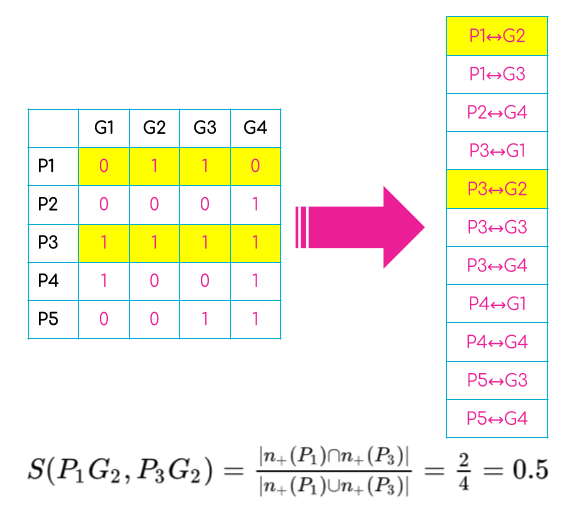
\includegraphics[width=1.0\textwidth]{Figs/Toy/link-clust-toy1.png}
        \caption{Two person-genre edges sharing the same genre.}
        \label{fig:link-toy1}
    \end{subfigure} 
     \begin{subfigure}[b]{0.3\textwidth}
        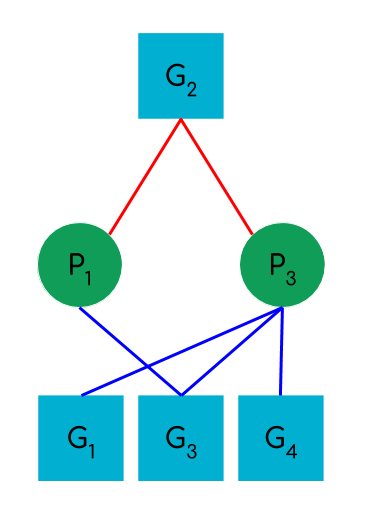
\includegraphics[width=1.0\textwidth]{Figs/Toy/link-clust-toy2.png}
        \caption{Similarity between person-genre edges depends on the other genres people are linked to.}
        \label{fig:link-toy2}
    \end{subfigure}
     \begin{subfigure}[b]{0.45\textwidth}
        \includegraphics[width=1.0\textwidth]{Figs/Toy/link-clust-toy3.png}
        \caption{Edge similarity matrix from toy example.}
        \label{fig:link-toy3}
    \end{subfigure}
     \begin{subfigure}[b]{0.45\textwidth}
        \includegraphics[width=1.0\textwidth]{Figs/Toy/link-clust-toy4.png}
        \caption{Edge distance matrix from toy example.}
        \label{fig:link-toy4}
    \end{subfigure}
     \begin{subfigure}[b]{0.6\textwidth}
        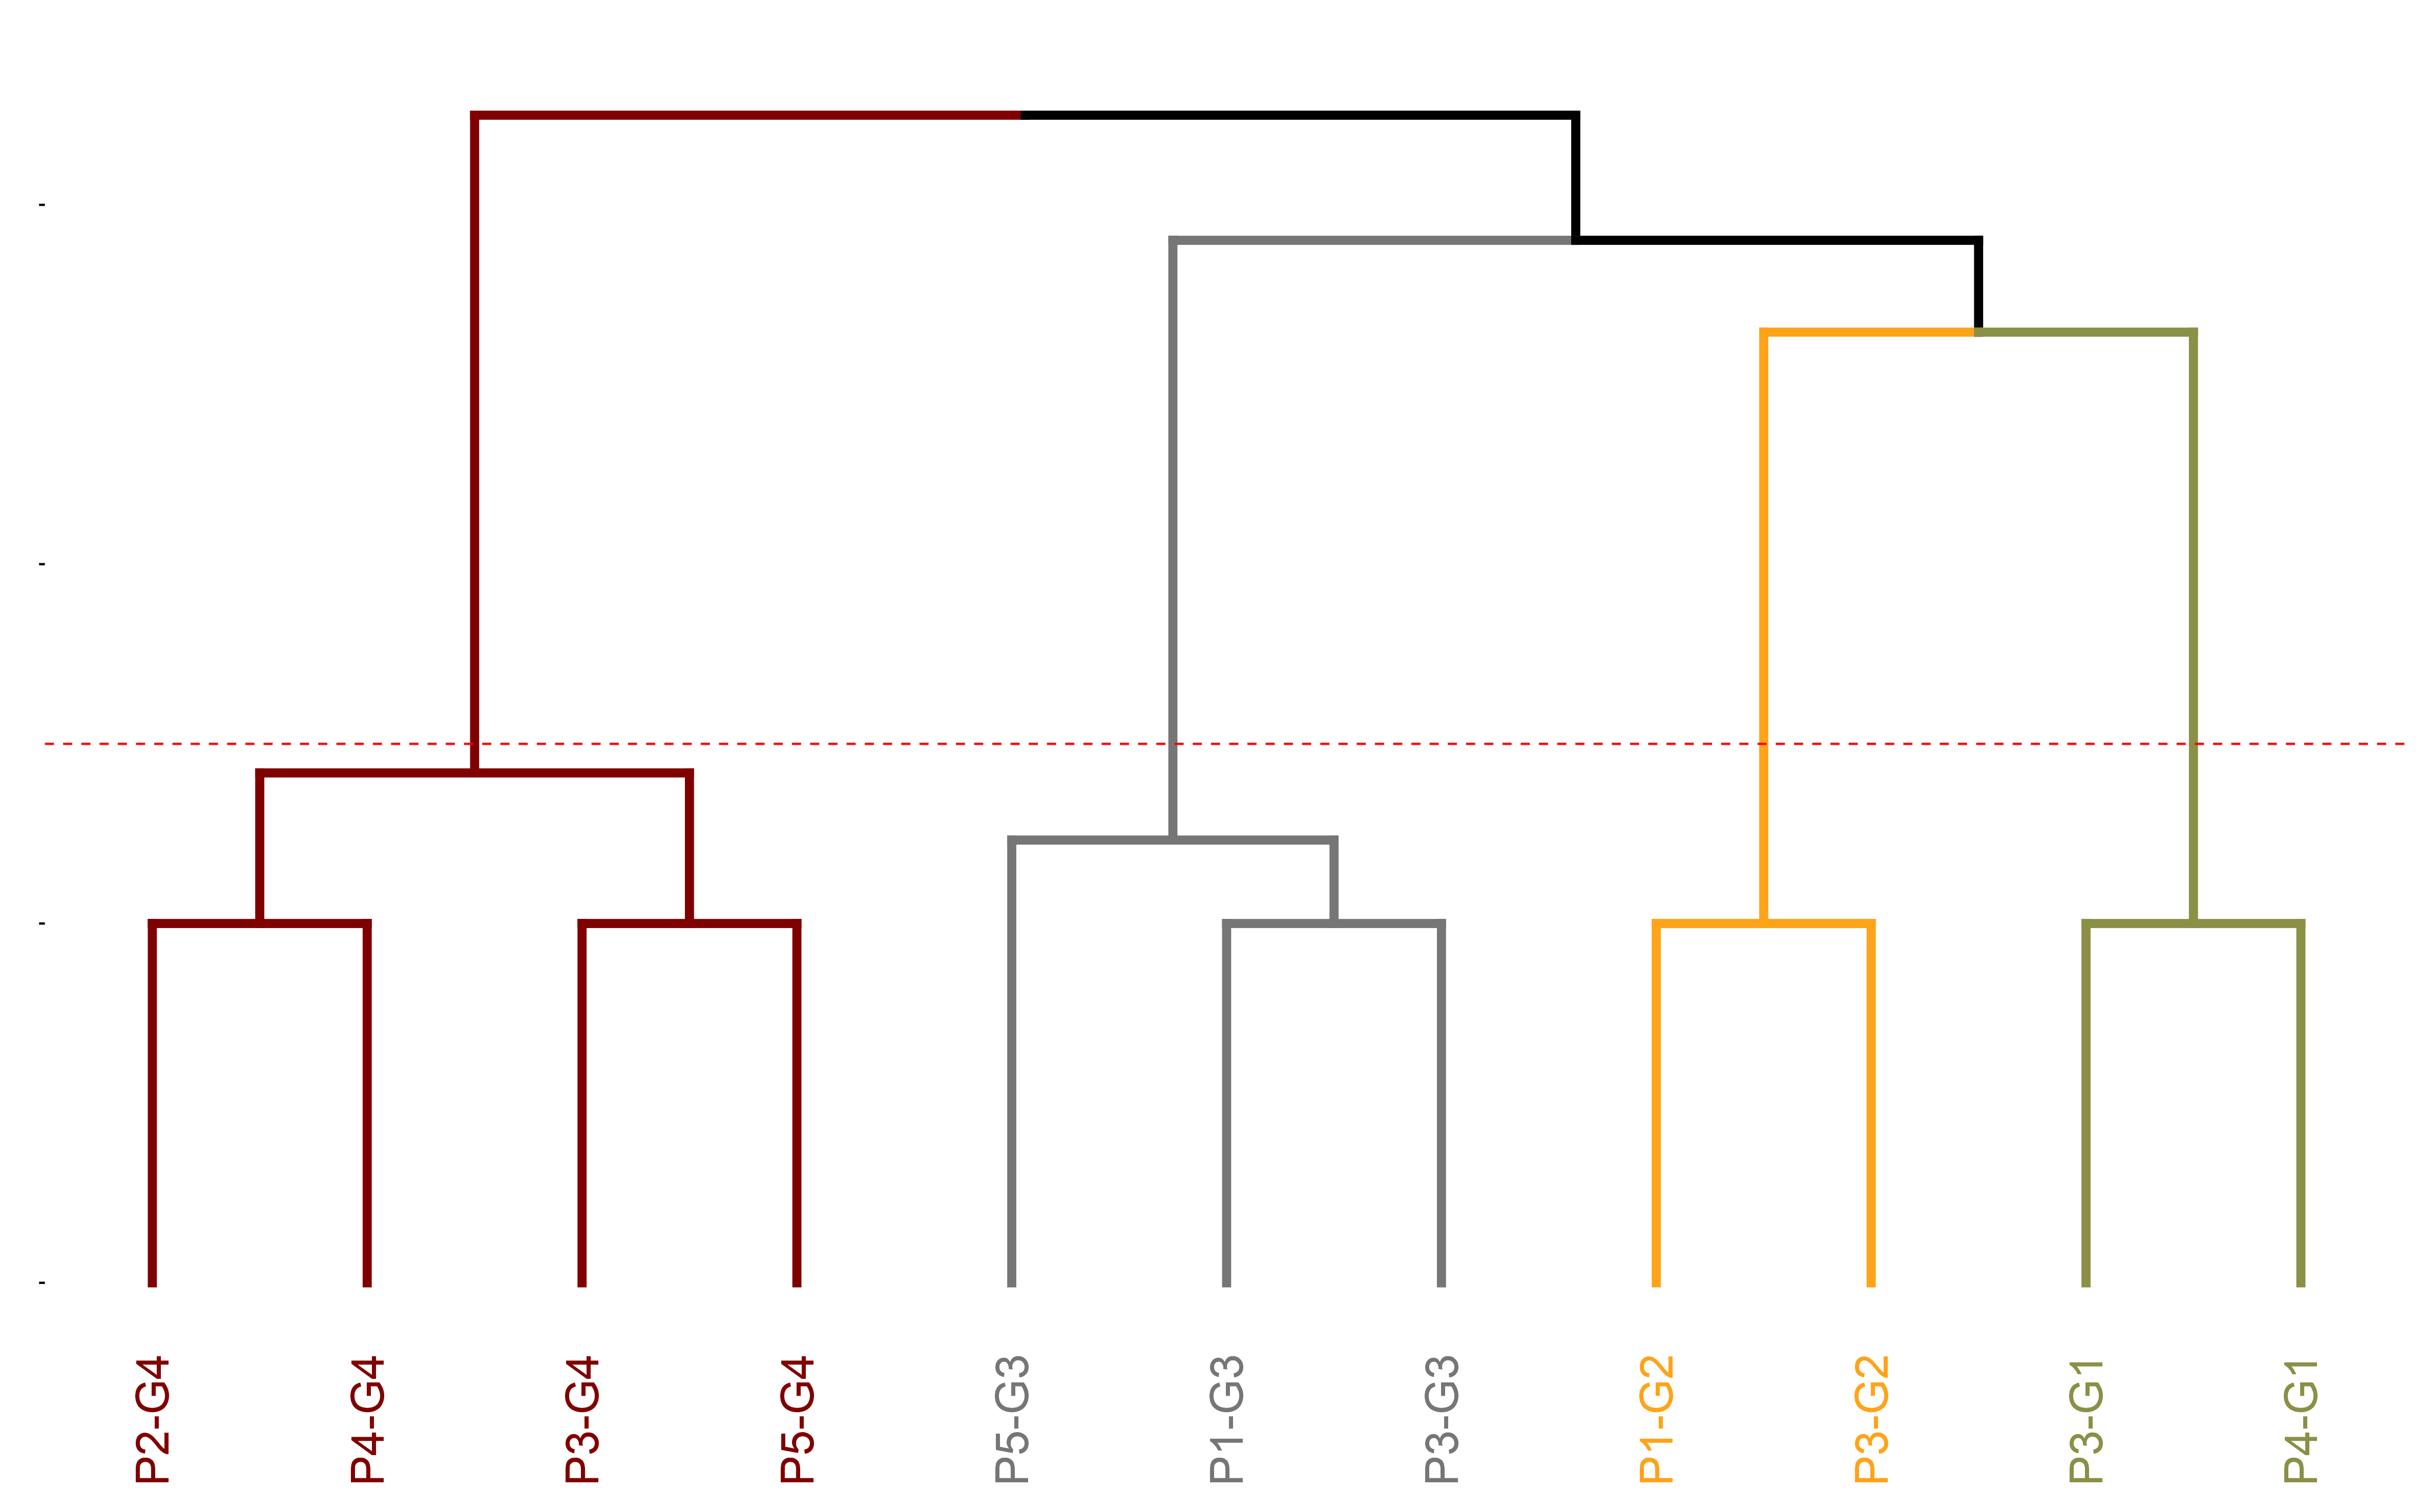
\includegraphics[width=1.0\textwidth]{Figs/Toy/link-clust-toy5.png}
        \caption{Dendrogram from Ward clustering of toy example edge distance matrix cut at four clusters.}
        \label{fig:link-toy5}
    \end{subfigure}
    \caption{Toy illustration of how the link clustering approach works.}
    \label{fig:link-toy}
 \end{figure}
 
How does this work? As Figure~\ref{fig:link-toy1} shows, once we string out the original two-mode person-by-network in our toy example into an edge list (now containing eleven person-genre edges), where the cases are the person to genre pairs that are marked by a ``1'' in the original matrix, it is possible to ask: ``How similar is one edge to another?'' We can answer that question as follows. The similarity of one person-to-genre edge to another, when both edges point to the same genre \citep{ahn_etal10}, should be proportional to the overlap between the ``cultural ego networks'' of the two people at the tail end of the edges. As \citet{lizardo14} defines it, for any respondent $i$, in a survey on cultural taste, the cultural ego network is simply the set of genres $\{G_1, G_2,\dots G_k\}$ chosen by the person. 

Going back to our running toy example, we are tasked with computing the similarities between $\frac{11 \times (11-1)}{2} = 55$ person to genre pairs. Suppose we wanted to calculate the similarity between the $P_1-G_2$ and $P_3-G_2$ person-to-genre edges in the two-mode network. In Figure~\ref{fig:link-toy1}, these two links are highlighted in yellow the ``strung out'' edgelist and are shown in red in the corresponding bipartite subgraph shown in Figure~\ref{fig:link-toy2}. The similarity ($S$) between the two links is then given by:

\begin{equation}
    S(P_1G_2, P_3G_2) = \frac{n_+(P_1) \cap n_+(P_3)}{n_+(P_1) \cup n_+(P_3)}
\end{equation}

Where $n_+(P_1)$ is the cultural ego network of Person 1 and $n_+(P_3)$ is the cultural ego network of Person 3. The formula says that the similarity between two person-to-genre links sharing a genre, in this case, the similarity between the $P_1-G_2$ edge and the $P_3-G_2$ edge, is given by the intersection of Person 1's and Person 3's cultural ego network divided by their union (also known as Jaccard's coefficient). When the cultural ego networks of two people are the same then $S=1$, when they are completely disjoint (share no genres, meaning the intersection is the empty set), then $S = 0$. All other cases of person-to-genre edges sharing the same genre return a number between zero and one ($0 > S < 1$).\footnote{Note that the only substantive similarities we care about are between person-to-genre edges that shared the same genre but have different people attached to them at the other end. All other person-to-genre edges, featuring people connected to different genres are set to zero.} In the toy example case, $P_1$ and $P_3$ consume two genres out of the four possible ones they could consume in common, resulting in an edge similarity score of $\frac{2}{4} = 0.50$. 

If we do that for all pairs of person-to-culture genres sharing one genre node in common, we end up with the two-way, one-mode (with the only mode being edges) $11 \times 11$ similarity matrix shown in Figure~\ref{fig:link-toy3}. Note two features of the similarity matrix. First, by definition, two person-to-genre links that go from different genres to the same person are maximally similar (as the overlap is 1.0). This means that only links that go from different people to the same genre exhibit overlap variation, and this is driven (``reflectively'' \citep{lizardo18}) by the overlap between the neighborhoods of the other mode (people). Next, we transform the similarity matrix into a {\em dissimilarity} matrix by subtracting one from each entry (shown in  Figure~\ref{fig:link-toy4}). We then subject this matrix to hierarchical clustering using Ward's \citeyearpar{ward63} method. 

The resulting dendrogram from the cluster analysis is shown in Figure~\ref{fig:link-toy5}. Note that moving from the top down, the dendrogram splits person-to-genre links according to the macrogenre label. That is, macrogenre information is preserved in the clustering and can be recovered by splitting the dendrogram at a height where the number of clusters is equal to the original number of macrogenres (in this case, four as shown in Figure~\ref{fig:link-toy5}). Moving from the bottom up, the hierarchical clustering of the dissimilarity matrix yields {\em link communities} \citep{ahn_etal10}, in which both people nodes, but, most crucially, genres nodes are assigned to different clumps. In the limiting case (the dendrogram's bottom-most ``leafs''), each person-to-genre link is assigned to a cluster. The more interesting thing is that as we move up to a point below macrogenres clusters and above the leaves, we see a partition of {\em varieties} of macrogenres. For instance, macrogenre $G4$ is split into two focused microgenre varieties. The first is attached to persons $P2$ and $P4$, and the second attached to persons $P3$ and $P5$, respectively. The idea, is that the macrogenre nodes (e.g., ``Classical,'') assigned to different clumps represent micro-variations of the macrogenre label that differ primarily relationally or structurally; different ``types'' of ``Classical'' are different because their audiences make distinct choices {\em with respect} to the other genres in the survey. 

\begin{figure}[ht!]
     \begin{subfigure}[b]{0.5\textwidth}
        \centering
        \includegraphics[width=1.0\textwidth]{Figs/Dend/all-branches-macro.png}
        \caption{c = 8, k = 20}
        \label{fig:dend-macro}
    \end{subfigure} 
     \begin{subfigure}[b]{0.5\textwidth}
        \centering
        \includegraphics[width=1.0\textwidth]{Figs/Dend/all-branches-macro-labels.png}
        \caption{c = 8, k = 20}
        \label{fig:dend-macro-labels}
    \end{subfigure} 
     \begin{subfigure}[b]{0.5\textwidth}
        \centering
        \includegraphics[width=1.0\textwidth]{Figs/Dend/all-branches-micro.png}
        \caption{c = 3, k = 102}
        \label{fig:dend-micro}
    \end{subfigure} 
     \begin{subfigure}[b]{0.5\textwidth}
        \centering
        \includegraphics[width=1.0\textwidth]{Figs/Dend/all-branches-micro-labels.png}
        \caption{c = 3, k = 102}
        \label{fig:dend-micro-labels}
    \end{subfigure}
     \begin{subfigure}[b]{0.32\textwidth}
        \centering
        \includegraphics[width=1.0\textwidth]{Figs/Dend/classic-rock-branches.png}
        \caption{c = 3, k = 12}
        \label{fig:dend-micro-classic-rock}
    \end{subfigure} 
     \begin{subfigure}[b]{0.32\textwidth}
        \centering
        \includegraphics[width=1.0\textwidth]{Figs/Dend/blues-branches.png}
        \caption{c = 3, k = 5}
        \label{fig:dend-micro-blues}
    \end{subfigure}
     \begin{subfigure}[b]{0.32\textwidth}
        \centering
        \includegraphics[width=1.0\textwidth]{Figs/Dend/opera-branches.png}
        \caption{c = 3, k = 2}
        \label{fig:dend-micro-opera}
    \end{subfigure}
    \caption{}
    \label{fig:dend}
 \end{figure}
 
The resulting partition has two interesting (and desirable) properties. First, the number of genre communities that \textit{people} belong to is deterministic, and it is given by the number of macrogenre labels they initially chose. Thus, link clustering preserves the cultural ego network degrees (omnivorousness by volume) of the people mode \citep{lizardo14}. Second, the number of microgenres into which the macrogenres are split is {\em not} deterministic. Instead, it is data-driven (discovered or learned) and cannot be pre-specified in advance. It is a function of relational information implicit in the overlap structure of the cultural ego networks of people in the data. Thus, link community detection of the person-to-genre network allows us to go from a situation starting with a person-to-genre network featuring a relatively small number of macrogenres and end up with an enlarged two-mode network with the same number of nodes in one mode (the people) but many more nodes in the other mode (the microgenres). How many microgenres ($N_m$) emerge is up to the analyst as it depends on where we ``cut'' the resulting clustering dendrogram. This will be somewhere between $N_g \geq N_m \leq N_l$, where $N_g$ is the number of original (macro) genres and $N_l$ is the number of person-to-genre links.

\section{Analysis and Results}
\subsection{Discovering microgenre Communities in Real Data}
Let us see how this process works in real data. We will see that link clustering can uncover valid microgenres. Recall that the data features 2,263 people choosing up to 20 macrogenre labels. When strung out as an edgelist, this results in 9,216 person-to-genre connections in the data, the resulting $9216 \times 9,216$ matrix, containing Jaccard similarities among person-to-genre links sharing a node in either of the two modes, is then the input to an agglomerative hierarchical clustering algorithm using Ward's \citep{ward63} method. The hierarchical clustering process proceeds as follows. 

Initially, each person-to-genre link is assigned to a singleton cluster. Then, in the second time step, the pairs of links with the largest Jaccard similarities are put in the same clump. This continues at each time step, where pairs of links with the largest similarity are chosen, and their respective communities are merged. This process is repeated until all links belong to a single cluster. The history of the clustering process is then stored in a dendrogram, which encodes all the information on the hierarchical organization of the genre communities. The height of the dendrogram provides information about the strength of the genre communities. As we have seen, the highest levels reproduce the original macrogenres, while the lower levels uncover more focused microgenres embedded within them. This is shown in Figure~\ref{fig:dend}. 

Figure~\ref{fig:dend-macro} shows that when we cut the dendrogram at a high level (e.g., $C = 8$), we reproduce the original twenty macrogenres we began with as the ``discovered'' link communities. As Figure~\ref{fig:dend-macro-labels} shows, the agglomerative link clustering procedure roughly arranges the macrogenre levels by their original popularity (number of person-to-genre links). From left to right, these are Classic Rock/Oldies, Pop/Top 40, Country, Classical, Easy Listening, Blues/R\&B, Contemporary Rock, Rap/Hip Hop, Jazz, Gospel, Dance/Club, Indie Alternative, Latin, Broadway/Musicals, Heavy Metal/Hard Rock, Reggae, Big Band, Folk, Bluegrass, and Opera. As shown in Figure~\ref{fig:dend-micro}, microgenre communities are produced by cutting the link clustering dendrogram at a lower level. Choosing a cutoff value of $c = 3$ results in $k = 102$ microgenre communities extracted from the original twenty macrogenre labels. Data scientists wring their hands about choosing a cut value when performing cluster analysis. One advantage of the link clustering approach is that we always know what we are doing because microgenres are strictly nested within the original macrogenres. On the other hand, choosing a smaller cut value produces finer-grained microgenres (perhaps at the expense of analytic tractability and interoperability), and selecting a higher value returns us to broader genre communities closer to the original macrogenre labels we began with (with the limiting case as shown in Figure~\ref{fig:dend-macro} being the original macro genre labels themselves). As Figure~\ref{fig:dend-micro-labels} shows, at any cut value $C$, the more popular macrogenres produce more microgenre communities, while the less popular ones produce a smaller number. For instance, as shown in Figure~\ref{fig:dend-micro-classic-rock}, at $c = 3$, the macrogenre ``Classic Rock/Oldies'' (the leftmost set of branches in the dendrogram in Figure~\ref{fig:dend-macro}) is split (at the point at which the branches intersect the red dashed cut line) into $k_{(CR)} = 12$ distinct micro-variations, while, as Figure~\ref{fig:dend-micro-opera} shows, the macrogenre ``Opera" (the rightmost set of branches in the dendrogram in Figure~\ref{fig:dend-macro}) is split into only $k_{(Op)} = 2$  microgenre communities. Figure~\ref{fig:dend-micro-blues} shows that ``Blues/R\&B'' falls somewhere in between, with $k_{(BRB)} = 5$  microgenre communities uncovered.

Each cut point in the dendrogram will have a microgenre size distribution $N$ associated with it. Lower cut points return a microgenre size distribution dominated by many microgenres with tiny ($N_{mg} < 10$) or trivial $N_{mg} = 2$ audiences. In this respect, although I have been using the labels ``macro'' and ``micro'' as if they referred to substantive or objective partitions, they are best interpreted as {\em relative} to a given classification level. Thus, microgenres are ``micro'' relative to the usual (perhaps ``basic'' in Rosch's \citeyearpar{Rosch1978-ue} sense) categorization level of vague macrogenre labels populating most arts participation surveys. But these may be micro, as we will see, relative to the (logics, discourses, schemas) meta-groupings that we generate when applying the usual suite of statistical and data reduction techniques (e.g., such as ``highbrow'' or ``Folk"). Further, at any given classification level, further microgenres will be nested within any given micro-partition. In this way, microgenre communities reflect a substantively valid way in which people partition the cultural world, whereby there is always the possibility of making finer-grained distinctions within fine-grained distinctions (e.g., ``old school rap," ``1980s old school rap,", ``early 1980s old school rap," and the like). 
 
\subsection{Two Genre Case Studies}
We have shown that we can perform a link clustering and that this clustering returns a nice set of microgenres nested within the usual macrogenres in the survey. But does this exercise result in any substantive gains? In this section, I show that the link clustering approach does allow you to extract new insights from old data. There are many ways we can proceed. I choose to present two ``case studies'' of macrogenre labels and the resulting microgenre variations returned by the link clustering procedure. My criteria were as follows: I selected a macrogenre label for which I could find some substantiated claim in the scholarly literature regarding possible microgenre variation. Naturally, general claims about microgenre variation apply to all macrogenre labels. Therefore, the ``substantiated in the scholarly literature" serves as a way to narrow the field. I settled on Heavy Metal and Latin/Spanish Music/Salsa using this criterion. I intended to identify macrogenre labels for which some sort of debate or uncertainty existed in the scholarly literature regarding their overall status and their variations. As we will see, Metal definitely fits this bill, as a lively debate already exists regarding its status. Latin/Spanish/Salsa represents a more ``minor'' case study in comparison but still serves to showcase the usefulness of the link clustering approach for resolving key issues.

\subsection{Heavy Metal}
Heavy Metal is one of the most storied macrogenre labels in the sociology of taste, as featured in the title of Bethany Bryson's \citeyearpar{bryson96} now classic paper. Since then, it has been the subject of scholarly debate regarding its possibly changing status in the cultural stratification order \citep{tampubolon2008revisiting, goldberg2011mapping, lizardo_skiles15}. Heavy Metal stood out in Bryson's study for several reasons. First, it was the most disliked genre in the 1993 General Social Survey culture module data---one of the most heavily analyzed data sources in the sociology of taste---hence the ``Anything But'' in the title of Bryson's eponymous piece. Second, it was the prototypical genre that was relatively more favored by working-class audiences but absolutely hated by individuals with high education. Thus, it served as the linchpin of Bryson's symbolic exclusion argument; omnivores were omnivorous up to a point, except when it came to those genres most favored by those with low education. 

Regardless, the picture we got of Metal concerning audience segmentation was clear: It was a genre that primarily appealed to working-class, low-education white men and was rejected by pretty much everyone else. Lizardo and Skiles \citeyearpar[][6, table 2]{lizardo_skiles16} used the same data source as in this paper (data from 2012) and found that, nineteen years later, Metal was still the most disliked of the macrogenre labels in a representative sample of Americans. Not only that, but when asked who the typical fan of metal looked like, Americans agreed with the stereotype: Low education, ``lower'' and working-class white men \citep[][7, table 3]{lizardo_skiles16}. 

Yet, cracks began to appear in this picture as soon as it was hung. First, Tampubolon \citeyearpar{tampubolon2008revisiting} re-analyzed the Bryson data using a different methodological approach (latent-class analysis), making different inclusion decisions regarding the ``don't know'' responses. Tampubolon shows that including those ``don't know'' responses significantly changes things. Concerning Metal, it indicates that it is strongly disliked among low-education people more than would have been surmised in Bryson's original study, so it is not just a top-down symbolic exclusion story. For Tampubolon, this makes Metal ``quite exceptional'' since it is disliked across the board and even more by low-education people. 

Tampubolon's work indicates that just because Metal's audience is composed of low-education people does not mean that the rest of the less-educated population loves it; in fact, they hate it passionately. Tampubolon's analysis of ``Like'' responses also shows that Metal, rather than being exclusively preferred by a univorous group of ``Metalheads'' (who only prefer metal and dislike everything else), also makes it into the taste profile of one of two omnivorous groups uncovered in his analysis. Thus, Metal ends up straddling omnivores and univores. Because of this, even in the 1993 GSS data, its association with markers of status was ambiguous, leading Tampubolon to conclude that ``[p]reference or dislike for heavy metal is, therefore, orthogonal to status as measured by education'' \citeyearpar[][257]{tampubolon2008revisiting}, and that ``heavy metal is definitely not a low culture in the sense of culture `strongly associated' or very much liked by those with low education'' (\textit{ibid}).

Tampubolon's argument regarding Metal dovetail with those preferred by Lizardo and Skiles \citeyearpar{lizardo_skiles15}, using the same data source as in this paper. Yes, while Metal was still the most disliked genre in 2012, \textit{compared} to 1993, it was one of the macrogenre labels (Rap and Hip Hop being the other) that experienced the steepest \textit{declines} in being disliked in the intervening two decades, especially among younger audiences. This led Lizardo and Skiles \citeyearpar[][18]{lizardo_skiles15} to conclude that ``The fact that young, highly educated Americans are now about as equally unlikely to dislike\ldots Heavy Metal as their same-age non-college educated peers constitutes a dramatic reversal of the pattern noted by Bryson\ldots [Metal] has experienced an improvement in standing among the college educated across almost all levels of age.'' This strongly suggests that enjoying some types of Metal music may be an ``emerging form'' of cultural capital \cite{prieur2013emerging} among certain segments of the young elite.  

\subsubsection{Microgenre Analysis}
So, will the real heavy metal please stand up? Is Metal a form of emerging cultural capital with potential appeal to young middle-class people or a genre heavily favored by white men with low education? Or is that an outdated picture of the American musical field? Is Metal even correlated with status markers like education at all, as Tampubolon suggested? Is speaking of Metal as a ``youth'' music accurate, or has its audience been aging along with the genre (going on more than four decades and counting)? Given prior work, a strong expectation is that, at the very least, we should observe a microgenre partition separating the ``prototypical'' Metal (appealing to low-education white men) and perhaps a less-prototypical one, appealing to younger audiences with high-level cultural capital with other micro-variations, perhaps track generational distinction \citep{lizardo_skiles15}.

\begin{figure}[ht!]
    \centering    
    
\includegraphics[width=1.5\textwidth]{Tabs/reg-tab-metal.png}
    \caption{}
    \label{tab:reg-metal}
\end{figure}
    
To examine these questions, I partitioned the Heavy-Metal branch of the dendrogram, at a height that resulted in four microgenre variations. To explore the issue of audience segmentation, I specify a linear probability regression model with five outcomes: First, a binary variable indicating that a person chose (liked and listened to) the standard macrogenre label (Heavy Metal), and then four models with the microgenre variations as the outcome (Heavy Metal one through four). The results are shown in Table~\ref{tab:reg-metal}. The main predictors are the respondent's education, an indicator variable for whether at least one of the respondent's parents has a college degree, the respondent's age, racial identification (in five categories), and gender identification (in two categories). Because the age effect is specified using a squared polynomial, it can be hard to interpret its substantive significance. To help with this, I show the predicted probabilities obtained for the model at different age values for the four different microgenres in Figure~\ref{fig:age-metal}.

\begin{figure}[ht!]
    \centering    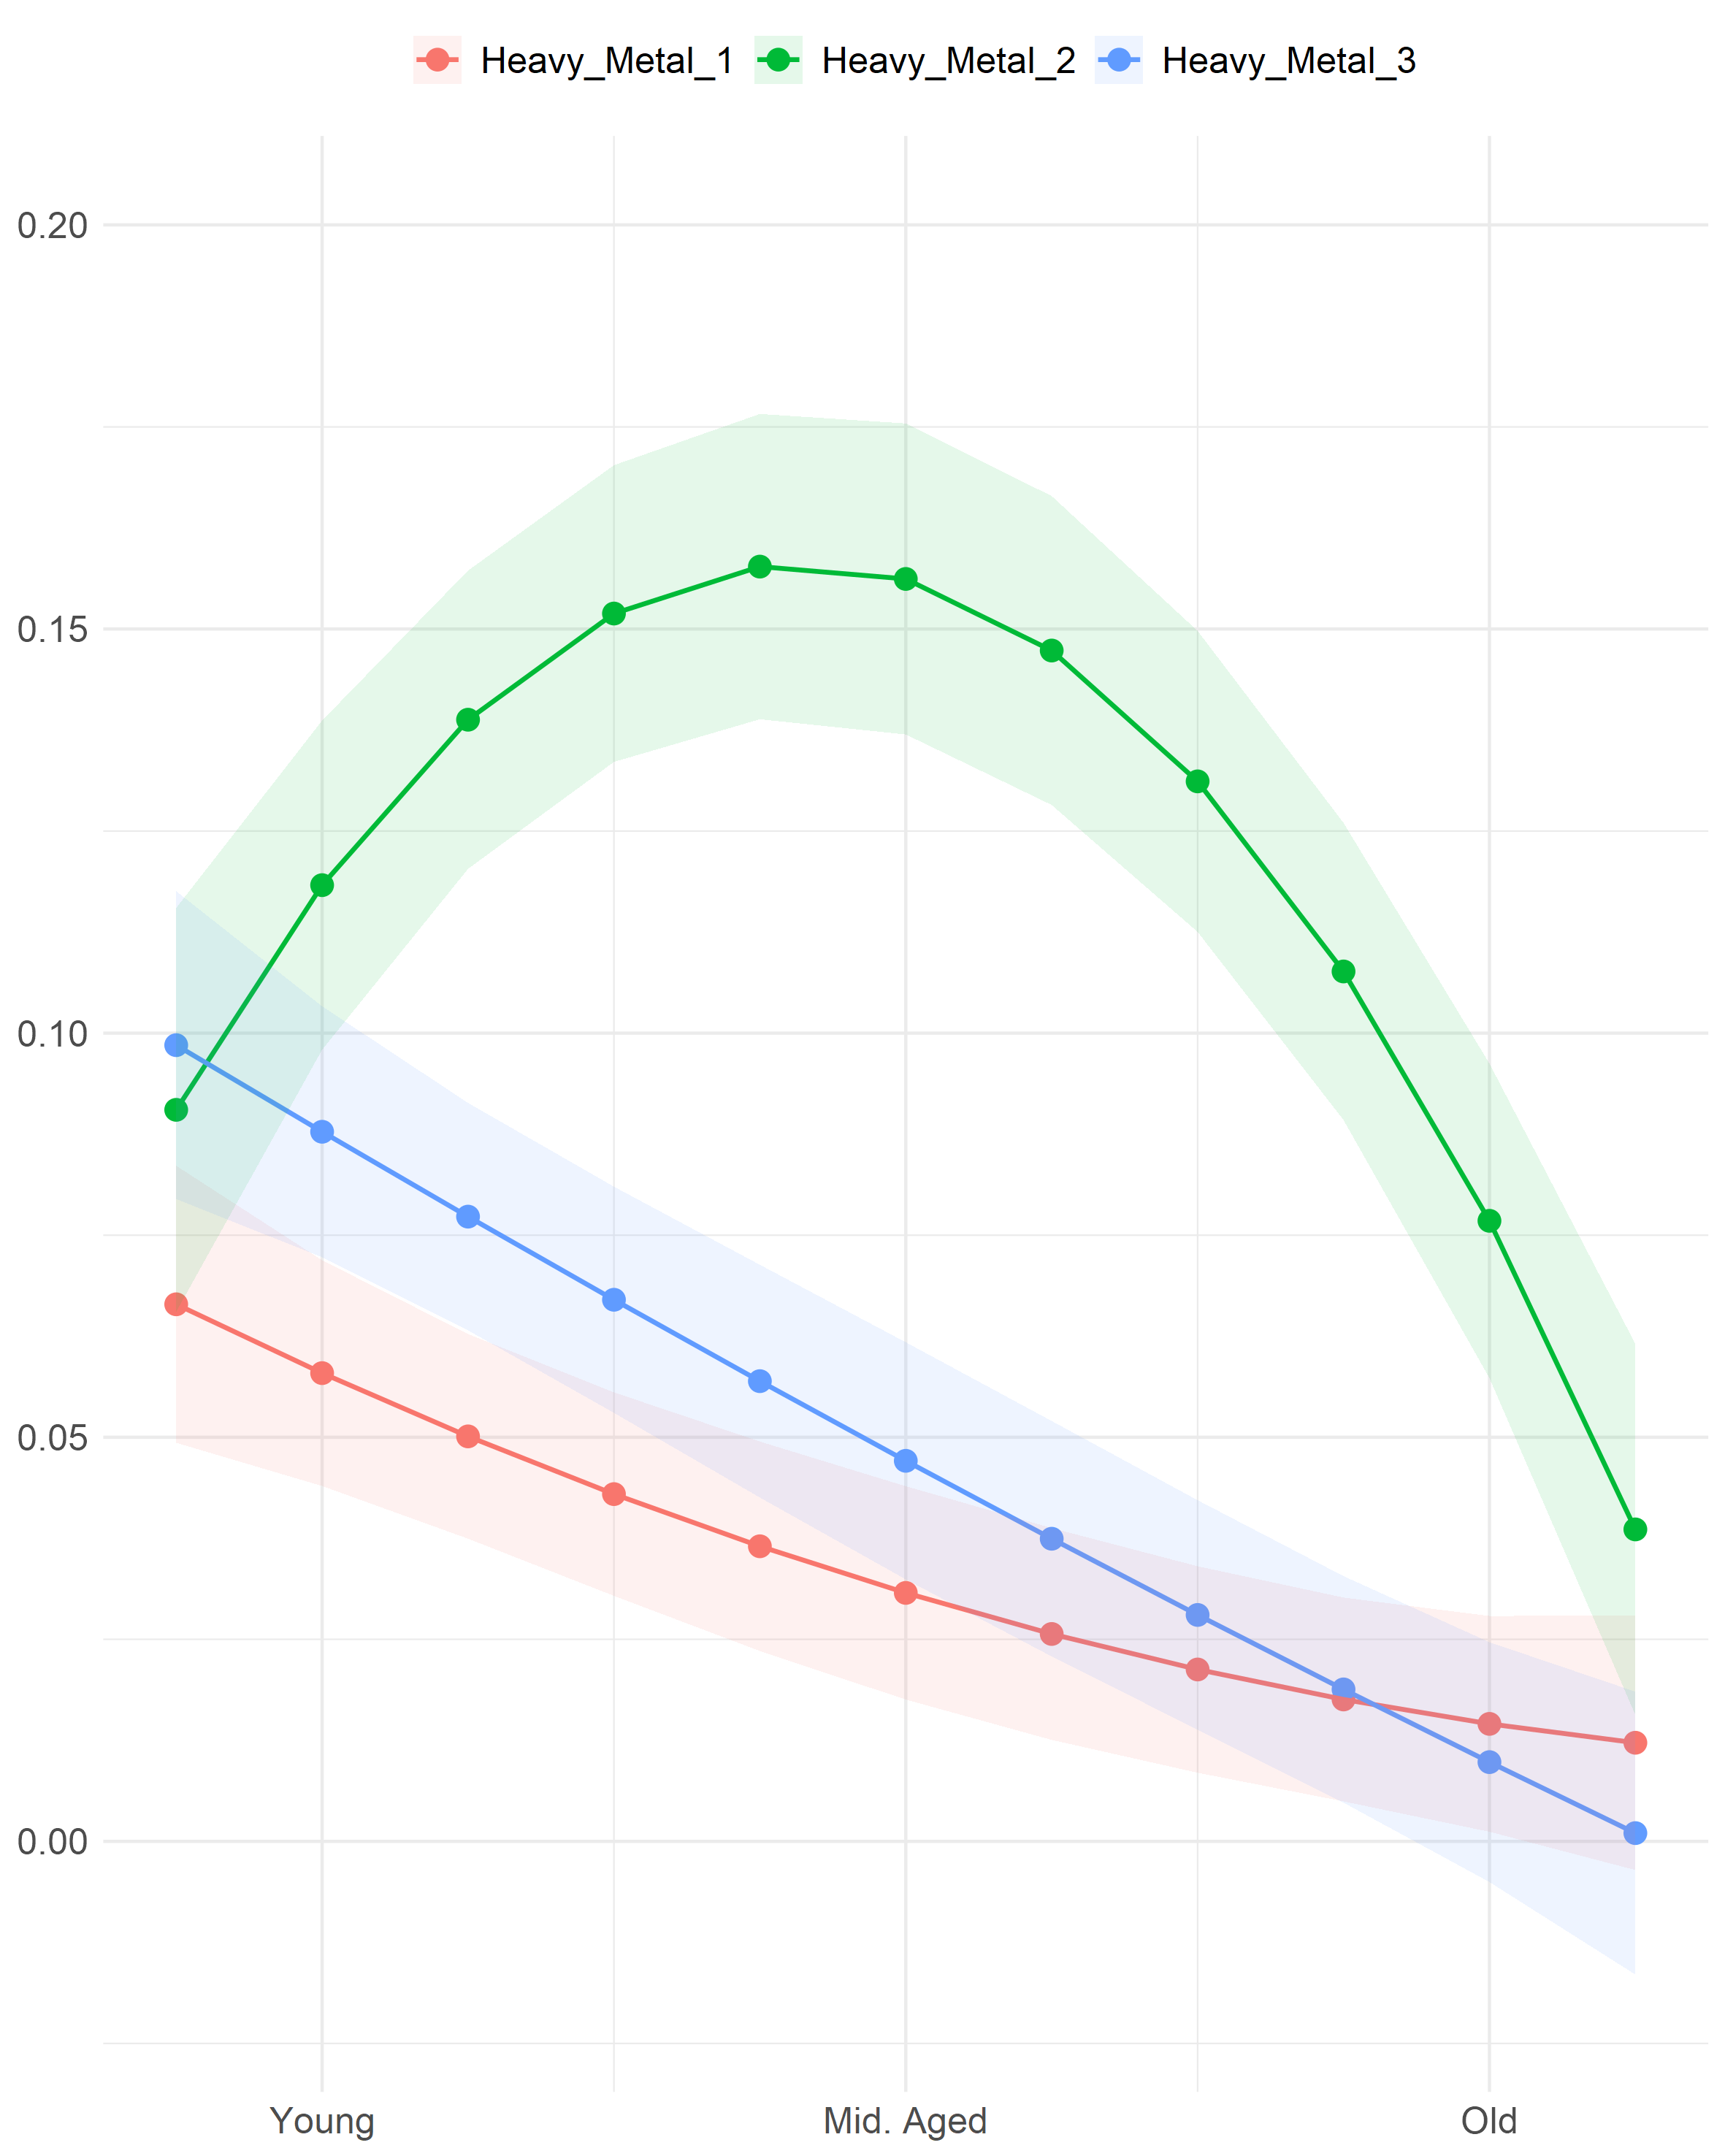
\includegraphics[width=1.0\textwidth]{Plots/Demog/micro-by-age-metal.png}
    \caption{}
    \label{fig:age-metal}
\end{figure}

As shown in the first model, the socio-demographic predictors of choosing the ``Heavy Metal'' macrogenre label are the ones we would expect from Bryson's original work and the stereotypical perception of the genre's audience held by Americans. Metal fans are less likely to have high levels of education, are less likely to be older, are more likely to be white (negative effects for all other racial identifications compared to the base category), and are more likely to be men ($p<0.01$). So much for the emerging cultural capital story?

Not so fast. The results differ when looking at the predictors of the microgenre variation choices. Indeed, the predictors of choosing the first microgenre variation, shown in the second column of the table, are consistent with Tampubolon's story. For this microgenre, there is a flat education gradient ($p = 0.54$), and importantly, it is more likely to be consumed by people whose parents have a college degree ($p < 0.05$), indicating a link to cultural capital in the home environment. This microgenre is tilted towards younger audiences, as only the linear negative age term is statistically significant (see Figure~\ref{fig:age-metal}) and is also neutral with respect to race and gender. This version of Metal appeals mainly to young middle-class respondents and does not repel women or non-white audiences, a stark difference from what we would have concluded from observing the macrogenre label effects. 

Note that the other microgenre variations conform most closely to the audience segmentation we would expect from the version of Metal that would appeal to ``univore'' consumers, indicating that the link clustering can be discerned between these variants. Particularly, the second microgenre, whose predictors are shown in the third column, seems to be the ``uber-Metal,'' at least regarding the stereotype. It has a negative education gradient ($p = 0.06$), appeals to young-adult and middle-aged audiences (see Figure~\ref{fig:age-metal}), and repels Black and Hispanic people as well as women. The other Metal microgenres are variations on the same theme: The third microgenre, as shown in the fourth column in the table, is like the second but appeals mainly to young audiences, and the fourth Metal microgenre is also similar to the second but appeals to a comparatively older crowd. So the remaining microgenre partitions seem to indicate variations within the ``univore'' consumption profile, perhaps indicative of distinctive versions of Metal with an appeal to different generational niches \citep{koch2020evolutionary}. 

\subsection{Salsa}
``it is plausible that increasing appreciation among high-status groups for a genre conventionally defined as ‘popular’ or ‘lowbrow’, will go hand in hand with its symbolic upgrading. And when a genre expands and spreads in terms of production, distribution and reception, it is likely to differentiate into distinct styles or subgenres. Under these conditions, it is to be expected that differential appreciations for different styles and forms within a given genre will develop, which may end up in a more or less clear hierarchy within this genre'' \citeyearpar[][62]{Bachmayer2014-pk}

``Taste in salsa music shows a strong internal, hierarchical order between ‘artistic’ versus ‘popular’ styles that is not only acknowledged and defined as such by experts and professionals within the field, but also structures the taste patterns of different social classes'' \citeyearpar[][62]{Bachmayer2014-pk}

\begin{figure}[ht!]
    \centering    
    
\includegraphics[width=1.5\textwidth]{Tabs/reg-tab-latin.png}
    \caption{}
    \label{tab:reg-metal}
\end{figure}

\begin{figure}[ht!]
    \centering    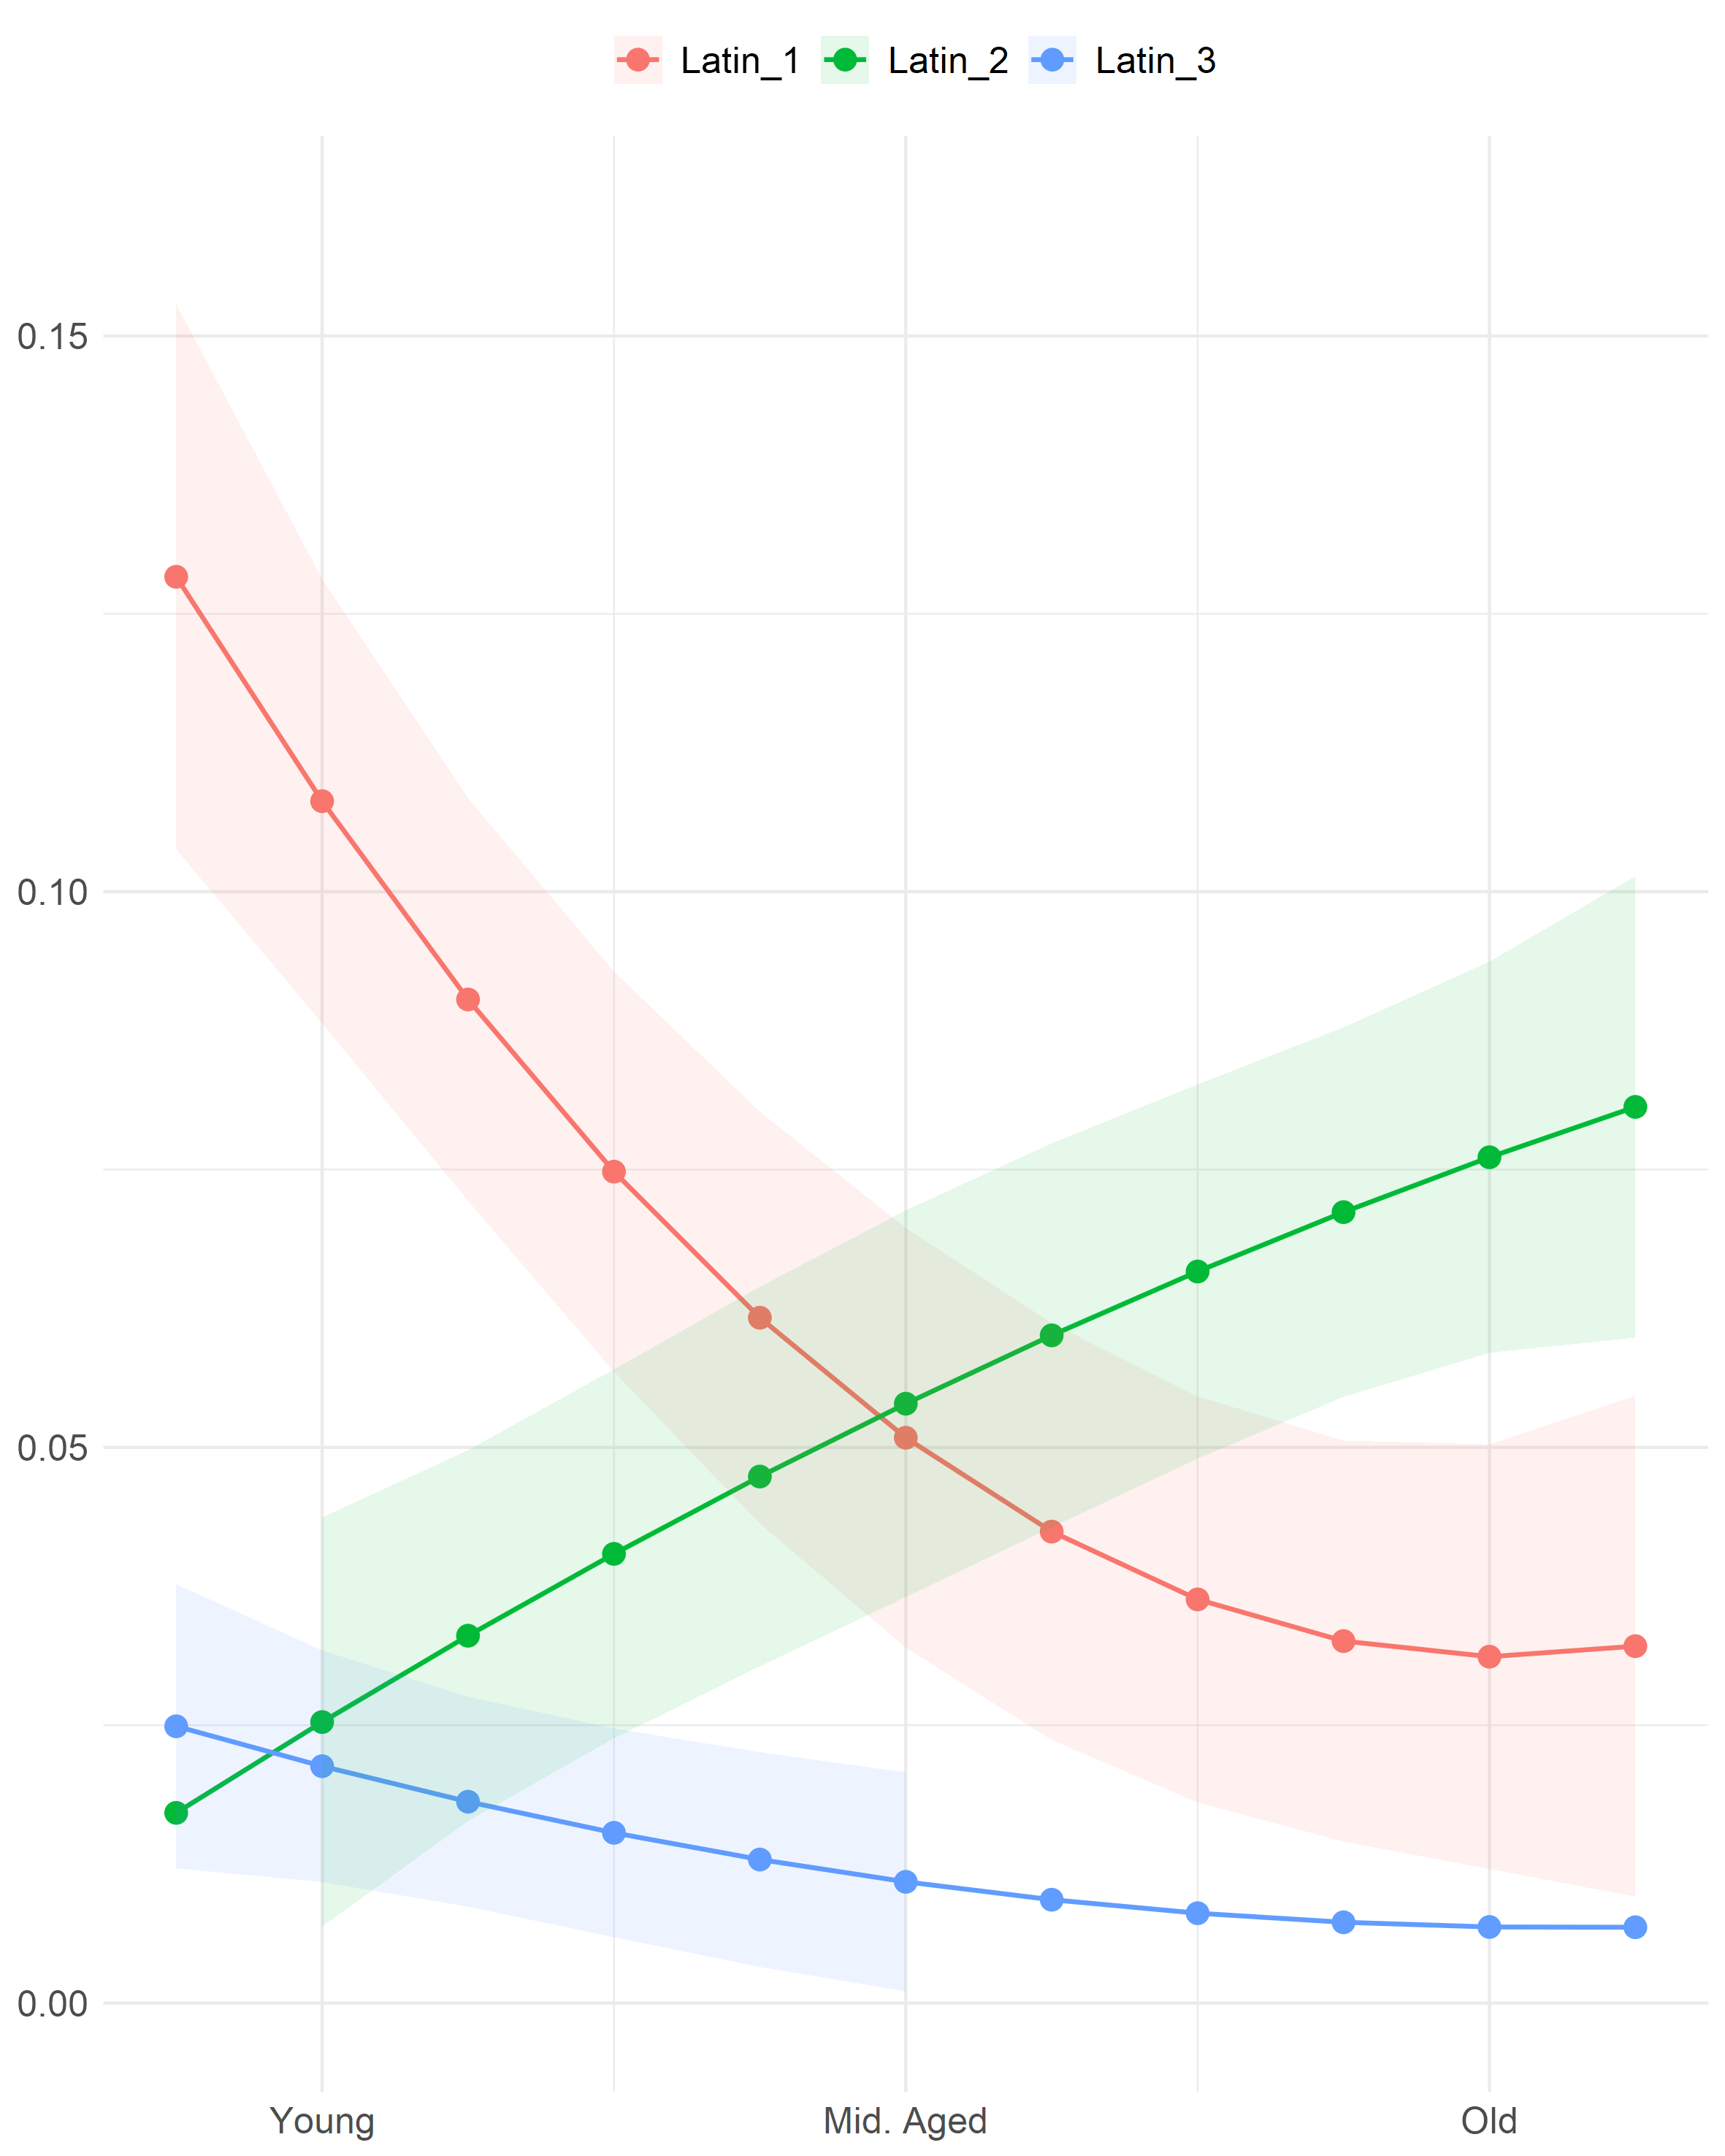
\includegraphics[width=1.0\textwidth]{Plots/Demog/micro-by-age-latin.png}
    \caption{}
    \label{fig:age-salsa}
\end{figure}

\section{Discussion}
Let us take stock. We began by discussing the network or ``relational'' revolution in the quantitative study of taste in sociology \citep{pachucki2010cultural}. We noted that many good things have come from considering survey data on taste using a relational lens, including a deeper specification of core concepts in the literature and even discovering new phenomena and empirical patterns. However, we also noted that survey data are as good as the labels chosen to collect the data. A resurgent line of critics questions whether the labels that appear in our most venerable survey-based studies are true ``genres'' in the sociological (or even stylistic) sense \citep{lena2015relational, vlegels2015music}. The labels are broad, likely to be interpreted by people in heterogeneous ways, and thus hide as much as they reveal. I noted recent attempts to just drop the idea of vague macrogenre labels and either study actual sociological genres on the ground (thus partially abandoning studies of audience segmentation or at least radically reconfigure them) or ``dropping the label'' \citep{sonnett2016ambivalence} by querying people about more focused objects of taste (e.g., performers within genres). These are all important and good developments, but we also noted that they may throw away a good thing. Upping the relationality by exploiting hidden patterns in the same old vague macrogenre-based data collected before can reveal focused microgenres. 

I proposed to do this using recent developments in the discovery of \textit{overlapping communities} in networks \citep{ahn_etal10}, which partially answers two of the challenges of macrogenre critics: The fact that actual genres are overlapping and not crisply bounded. The fact that there is hidden heterogeneity within the broad labels we usually focus on. Our analysis contrasted the application of the usual techniques to the same data, conceived in the usual ``macro" way, and \textit{after} upping the relationality and discovering the microgenres hidden within. It is clear that focusing on microgenres reveals variation and patterns of cultural choice (as well as audience segmentation) that we would not have noticed using the standard approach (in this, the critics are right). Still, we could do this without dropping the label or querying people about hundreds of micro-styles (most of which they'd be unfamiliar with). Instead, we exploited the venerable principle, etched into classical approaches to defining genres in network terms \citep{dimaggio1987classification}, noting that if genres are defined by the people who choose them, then they are also defined by the other choices that people make when they choose them; the country that combines with one version of Classical may not be the same country that combines with a version of the Blues (and neither is the same as the country that refuses to combine with any other style). 

The approach here is general and can be applied to studying other genre complexes beyond musical taste (allowing for economic data collection) and to studying other processes beyond taste. This includes belief, opinion, and attitude data. Essentially allows us to move from ``vague'' responses to more focused responses by exploiting the hidden patterns in the inter-response network formed when people respond to other items. Overall, we also learned a general lesson concerning our usual people or item classification techniques: To the extent that these are applied to items that themselves are ``vaguely'' defined, they will also yield even vaguer (and perhaps less than useful) macro-classifications of those items (like ``popular'' and ``high status''). The same may be said for such macro-classifications of opinions such as ``liberal'' and ``conservative,'' which, while being the primary way we interpret how people split themselves into groups by the beliefs they choose to hold, is decreasingly apt today if they ever were. 
 

\bibliography{refs.bib}
\end{document}
